\documentclass{article}
\usepackage{graphicx}
\usepackage[ngerman]{babel}
\usepackage{tipa}
\usepackage{natbib}
\usepackage{pdfpages}
\usepackage[utf8]{inputenc}

\begin{document}

\graphicspath{ {../images/} }

\begingroup
\centering
\vfill
\Large{Eine Vertiefungsarbeit über}\\
\Huge{KÜNSTLICHE SPRACHEN}\\
\huge{und}\\
\huge{MINIMALISTISCHE SPRACHEN}\\
\large{für die}\\
\Large{Technische Berufsschule Zürich}\\
\vspace{2cm}
\Large{von Samuel Pearce}\\
\vspace{1cm}
\large{Klasse AP18a}\\
\large{Abt. IT}\\
\large{Marlene Baeriswyl}\\
\vspace{1cm}
\Large{14.12.2021}\\
\vfill\null
\endgroup
\thispagestyle{empty}

\renewcommand{\abstractname}{Abstrakt}

\begin{abstract}
    Im Laufe meiner VA habe ich versucht, die Beziehung zwischen dem Umfang einer Sprache
    (d.h. der Anzahl der allgemein gebräuchlichen Wörter und der Komplexität ihrer Grammatik)
    und ihrer Verwendbarkeit im Alltag zu entdecken und besser zu verstehen.
    Zu diesem Zweck habe ich eine Weile damit verbracht, meine eigene Sprache von Grund auf zu
    entwickeln und einige Texte in diese Sprache zu übersetzen. Dann habe ich die Texte an meine
    Freunde weitergegeben, die versucht haben, sie ins Englische zurück zu übersetzen.
    So konnte ich feststellen, wie schwer die Sprache zu verstehen ist.
    Letztendlich waren die Experimente aus Zeitgründen nicht so ausführlich,
    wie ich es mir gewünscht hätte, aber die wichtigsten Schlussfolgerungen waren,
    dass eine Sprache mit einer sehr einfachen Grammatik bemerkenswert schnell erlernt
    werden kann und dass sogar sehr kleine Lexika für die meisten Situationen im Leben verwendet werden können.
\end{abstract}
\pagebreak

\tableofcontents
\pagebreak



\section{Einführung und Projektbeschreibung}
\subsection{Vorwort}
Ich habe dieses Thema gewählt, weil mich Sprache einfach sehr fasziniert und ich mich schon immer besonders
für die Idee der Sprachschöpfung interessiert habe. Ich möchte diese Gelegenheit auch nutzen,
um den Subreddits ``r/linguistics'', ``r/conlangs'' und ``r/neography'' dafür zu danken, dass sie dazu beigetragen haben,
die Liebe zu und das Verständnis für die Entstehung von Sprache zu fördern.
Und natürlich möchte ich mich vor allem bei meinen beiden Freiwilligen Amin Haidar \& Julian Werner
für ihre Hilfe und Geduld bei diesem Projekt herzlich bedanken.

\subsection{Kurze Erklärung der UG Theorie}
In der Linguistik ist das Konzept der ``Universellen Grammatik'' auch heute noch ein heiss diskutiertes Thema.
Diese Theorie besagt, dass jeder Mensch von Geburt an die gleiche Grundstruktur für Sprache in seinem Gehirn hat.
Die moderne Form der Theorie besagt, dass es keine festen Regeln gibt, die für jede Sprache gelten,
sondern dass es Prinzipien gibt, die für jede Grammatik gelten, die aber durch Parameter angepasst werden,
was zu der fast fraktalen Komplexität aller Sprachen der Welt führt. Ein Beispiel hierfür wäre das mögliche Prinzip,
dass Satzbewegungen nur auf einen kurzen Bereich beschränkt sind, und ein Beispiel für einen Parameter ist der ``Head-Parameter'',
der vorschreibt, in welcher Reihenfolge Phrasen im Verhältnis zu ihrem ``Kopf'' gebildet werden.\citep{ChUGAI}

Der Grund, warum die Universalgrammatik eine so schwer zu knackende Nuss ist, liegt darin, dass Sprache etwas extrem Subjektives
ist und dass es --- zumindest solange wir das Geheimnis des menschlichen Bewusstseins nicht gelüftet haben --- unmöglich ist,
genau zu wissen, was jemand bewusst oder unbewusst zu einem bestimmten Zeitpunkt denkt. In meinem letzten Aufsatz,
in dem ich mich auf die Theorie der Universalgrammatik konzentrierte, sprach ich mich für die Verwendung konstruierter Sprachen aus,
um zu erproben, was mit der menschlichen Sprache möglich ist, und um die Tiefen unserer Sprachfähigkeiten auszuloten.

Deshalb habe ich mich entschlossen, die mir für dieses Projekt zur Verfügung stehende Zeit (und einen beträchtlichen
Teil meiner Freizeit) damit zu verbringen, die Funktionsweise von Minimalsprachen besser zu verstehen,
nachdem ich mich für das Konzept von Toki Pona, einer Sprache mit nur etwa 130 Wörtern und 7 Grammatikregeln\citep{Lang14},
begeistert hatte. Obwohl ich zugeben muss, dass dies wenig mit der Universellen Grammatik zu tun hat,
könnte es einige universelle Regeln in Bezug auf die Grösse des Lexikons und den Punkt,
an dem Abstraktion zu mehrdeutig wird, aufdecken.

\subsection{Prozess der Spracherstellung}
Zu Beginn meiner VA und als Vorbereitung darauf begann ich, mich mit der Phonologie und Grammatik der Sprache zu beschäftigen.
Aus persönlichem Interesse verfügte ich bereits über einige Kenntnisse und Erfahrungen mit dem Prozess der Sprachentwicklung.
Ich hatte an vielen Online-Foren teilgenommen, die sich mit konstruierten Sprachen, der Konstruktion von Sprachen und der
Linguistik im Allgemeinen befassten. Der erste Schritt bestand darin, die Phonologie zu konstruieren, d. h. die Laute,
die in der Sprache verwendet werden sollten. Das war ein ziemlich einfacher Schritt, da ich mir darüber schon seit einiger
Zeit Gedanken gemacht hatte und die einfache Phonologie, die ich mir bereits ausgedacht hatte, nur noch geringfügig ändern musste.
Ich fügte auch ein System von Umlauten ein, das auf der Rundung der Vokale basiert. Dies bedeutete, dass 3 der 4 Vokale
in der Sprache von ihrer ``weichen'' Form (ungerundet für vordere Vokale und gerundet für hintere Vokale) zu ihrer ``harten'' Form
(das Gegenteil) wechseln konnten. Der Grund für den Unterschied zwischen vorderen und hinteren Vokalen war, dass vordere Vokale
in der Regel ungerundet sind, während hintere Vokale normalerweise gerundet sind.\citep{Stevens72} Durch die Abstraktion
``hart''/``weich'' klang es für die erwarteten Sprecher (Deutsch-/Englischsprecher) natürlicher.

Danach begann ich mit verschiedenen grammatikalischen Strukturen zu experimentieren und zu überlegen,
wie man sie umsetzen könnte. Obwohl dies für die Einfachheit der Sprache vielleicht keine gute Idee war,
gefiel mir die Idee, ein Kasussystem einzuführen, um der Sprache eine freie Wortfolge zu geben.
Das habe ich mit einfachen Suffixen gemacht, die den germanischen Kasusendungen nicht ganz unähnlich waren,
um die Mühe des Lernens auszugleichen. Danach wurde in ähnlicher Weise ein simples Zeitformsystem mit einfachen Suffixen
für Vergangenheit, Gegenwart und Zukunft aufgebaut. Der Aspekt wurde vorerst weitgehend vernachlässigt, da er später
möglicherweise durch Hilfsadverbien ausgedrückt werden könnte.

Nachdem sich die ersten Ansätze einer Grammatik herauskristallisiert hatten, überlegte ich mir,
wie ich den erforderlichen Wortschatz reduzieren könnte, um die wenigen Wörter, die ich definieren wollte,
optimal zu nutzen. Ein Gedanke, der mir kam und absolut Sinn machte, war ein konsonantisches Wurzelsystem wie im Arabischen
oder Hebräischen, begleitet von der Idee, eine Form der Wortumkehrung einzubauen, um die Bedeutung umzukehren, d. h.,
wenn man die Wurzeln eines Wortes umkehrt, würde es sein Antonym bilden. Beides zusammen würde bedeuten, dass jemand,
der die Sprache lernt, nur eine Wurzel lernen muss und daraus bis zu 6 Bedeutungen ableiten kann.

\begin{figure}
	\centering
	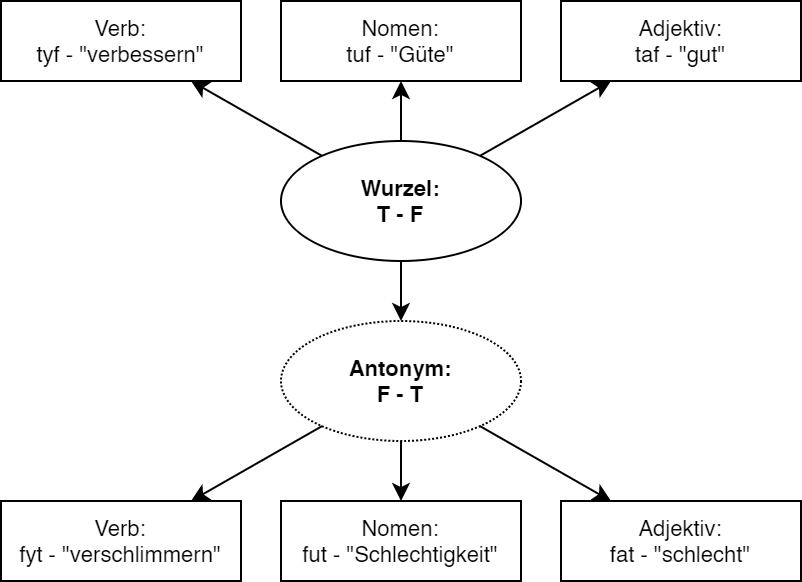
\includegraphics[scale=0.33]{root_derivations_1.png}
	\caption{Ein Diagramm aller Ableitungen der Wurzel ``T-F'' mit Inversion und dem bikonsonantischen Wurzelsystem.}
	\label{root_derivations_1}
\end{figure}

Da das Wurzelsystem nun einen bestimmten Vokal einer bestimmten Wortart zuordnet, können wir ihre ``harten'' Formen verwenden,
um einige semantische Veränderungen anzuzeigen. Ich beschloss, dass die reguläre Form die indikative Stimmung für Verben,
die Singularzahl für Substantive und der positive Grad für Adjektive sein würde. Für die Umlautformen entschied ich mich
für den Imperativ für Verben, den Plural für Substantive und den Superlativ für Adjektive. Dadurch verdoppelt sich die Anzahl
der Formen, die man aus einer einzigen Wurzel extrahieren kann.

\begin{figure}
	\centering
	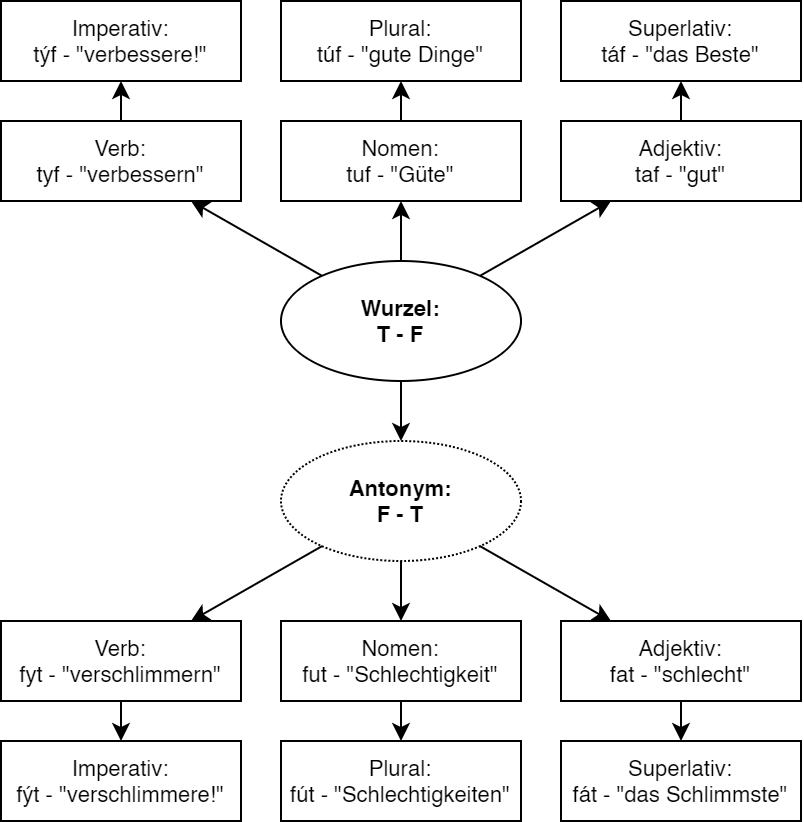
\includegraphics[scale=0.33]{root_derivations_2.png}
	\caption{Ein Diagramm aller Ableitungen der Wurzel ``T-F'' wenn mann die Umlautformen dazufügt.}
	\label{root_derivations_2}
\end{figure}

Danach wollte ich das System noch weiter ausbauen und schuf einige Präfixe, die unabhängig von der Wortart des Wortes
verwendet werden konnten. Diese würden es dem Sprecher ermöglichen, die möglichen Bedeutungen noch zu erweitern.
Zunächst wurden ein Negationspräfix sowie ein Augmentativ und ein Diminutiv hinzugefügt. Da diese auf alle vorhandenen
Ableitungen angewandt und sogar kombiniert werden können, vervielfachte sich die Zahl der möglichen Bedeutungen,
die einem einzigen Wort entnommen werden können, auf 60! Und dabei ist noch nicht einmal berücksichtigt,
dass die meisten Wörter absichtlich mehrdeutig sind, damit sie für mehrere Dinge stehen können. Zunächst war dies recht hilfreich,
um die Anzahl der Wörter zu reduzieren, die ich der Sprache hinzufügen musste, aber es wurde ziemlich schnell klar,
dass dies jeden Lernenden der Sprache nur verwirren würde. Zumal die Haupttaktik bei der Wortbildung darin bestand,
zunächst zu versuchen, das Wort aus anderen Wörtern zusammenzusetzen (z. B. ``Regen'' = ``fallende Flüssigkeit''),
aber obwohl ich in der Tat es geschafft hatte den Wortschatz sehr begrenzt zu halten, glaubte ich nicht, dass irgendjemand ausser mir sie
verstanden hätte. Ich habe dies auch getestet, indem ich meinen Freiwilligen ab und zu zusammengesetzte
Wörter zum Übersetzen vorgelegt habe. Die meisten Antworten bestätigten meine Befürchtungen, so dass ich eine Idee entwickelte,
um die Testkapazität der Sprache zu verbessern und gleichzeitig meine Angst vor dem Hinzufügen neuer Wörter zu überwinden:
Ich würde das Lexikon in kleine Segmente aufteilen, wobei die kleinste Ausgabe der Sprache nur die grundlegenden
grammatikalischen Wörter und eine Handvoll anderer enthalten würde. Danach würde der Umfang des Lexikons allmählich zunehmen,
bis er ein Maximum erreicht, das ich immer noch relativ klein halten wollte. Auf diese Weise könnte ich möglicherweise
Texte in immer kleinere Editionen der Sprache übersetzen, um zu sehen, an welchem Punkt genau sie jeden Anschein von
Bedeutung verliert. Ich beschloss, mir nicht allzu viele Gedanken über die Hinzufügung unnötiger Wörter zu machen,
da ich sie später immer noch einschränken und das Lexikon unterteilen konnte, sobald ich die gesamte Sprache etabliert hatte.
% TODO: Add in here if you do actually finish the Lexicon Size thing

Nachdem diese Grundlage mit dem Gerüst unserer Sprache ausgestattet war, konnte ich mich an die fortgeschritteneren
grammatikalischen Dinge wie Konditionalsätze und Relativsätze machen. Diese habe ich ähnlich wie bei Toki Pona gelöst,
weil es einfach zu verstehen ist und ich keine Zeit damit verschwenden wollte, mir etwas Besseres einfallen zu lassen.
Als ich das Ergebnis hatte, testete ich es an einigen Sätzen und befragte meine Testpersonen, was sie davon hielten und
ob ich ihrer Meinung nach etwas hinzufügen oder entfernen sollte. Sie hatten im Allgemeinen recht wenig Feedback,
und so hielt ich es für den Moment für gut genug und habe lediglich kleine Details verbessert und Wörter hinzugefügt/geändert,
als ich weitere Testsätze schrieb und kurze Texte übersetzte.

\subsection{Prozess der Sprachprüfung}
Zu Beginn des Projekts hatte ich weitaus ehrgeizigere Erwartungen, was das Testen der Sprache anbelangt,
aber im Laufe der Entwicklung wurde klar, dass ich das Testen der Fähigkeiten der Sprache einschränken sollte.
Schon bald wurde das Versuchskonzept auf die folgenden Punkte reduziert: Zuerst würde ich einen grösseren Textblock in die
Sprache übersetzen, danach würde ich meinen Freiwilligen dasselbe Wörterbuch zur Verfügung stellen, das ich für die Übersetzung
verwendet hatte, und ihre Fragen zur Grammatik beantworten, während sie den Text zurück ins Englische übersetzten.
Auf diese Weise konnte ich die Sprache testen und verfeinern, indem ich den grösseren Text übersetzte und so herausfand,
wie einfach es ist, die Bedeutung komplexerer Konzepte in der Sprache zu vermitteln, und meine Freiwilligen konnten zeigen,
wie gut man sie verstehen kann. Der Text, für den ich mich schliesslich entschied, war die Geschichte vom ``Turmbau zu Babel''
--- ein Favorit in der conlang Gemeinschaft. Hier ist der vollständige Text der Geschichte auf Deutsch:

\begin{quotation}
    Die ganze Erde hatte eine Sprache und ein und dieselben Worte.
    Als sie ostwärts aufbrachen, fanden sie eine Ebene im Land Schinar und siedelten sich dort an.
    Sie sagten zueinander: Auf, formen wir Lehmziegel und brennen wir sie zu Backsteinen.
    So dienten ihnen gebrannte Ziegel als Steine und Erdpech als Mörtel.
    Dann sagten sie: Auf, bauen wir uns eine Stadt und einen Turm mit einer Spitze bis in den Himmel!
    So wollen wir uns einen Namen machen, damit wir uns nicht über die ganze Erde zerstreuen.
    Da stieg der HERR herab, um sich Stadt und Turm anzusehen, die die Menschenkinder bauten.
    Und der HERR sprach: Siehe, ein Volk sind sie und eine Sprache haben sie alle.
    Und das ist erst der Anfang ihres Tuns. Jetzt wird ihnen nichts mehr unerreichbar sein, wenn sie es sich zu tun vornehmen.
    Auf, steigen wir hinab und verwirren wir dort ihre Sprache, sodass keiner mehr die Sprache des anderen versteht.
    Der HERR zerstreute sie von dort aus über die ganze Erde und sie hörten auf, an der Stadt zu bauen.
    Darum gab man der Stadt den Namen Babel, Wirrsal, denn dort hat der HERR die Sprache der ganzen Erde
    verwirrt und von dort aus hat er die Menschen über die ganze Erde zerstreut.\citep{Bibel2020}
\end{quotation}

Ursprünglich hatte ich auch geplant, Testgespräche mit meinen Freiwilligen zu führen,
aber sie waren zu dieser Zeit viel zu sehr mit ihren eigenen Projekten beschäftigt, um eine ganze Sprache zu lernen,
und wir konnten uns während der Pandemie nicht mehr treffen. Hätten wir es dennoch getan, wäre meine ursprüngliche
Idee für das Experiment gewesen, eine kurze Zeit unseres normalen Lebens damit zu verbringen,
die grundlegenden Dinge zu beschreiben, die wir tun, und uns normal in der Sprache zu unterhalten.
Das wäre meiner Meinung nach der beste Weg gewesen, um die Fähigkeit der Sprache zu testen, alltägliche Dinge auszudrücken.
Das System des skalierenden Lexikons könnte auch verwendet werden, indem man die Konversation zunächst auf das kleinste
Lexikon beschränkt und den Umfang allmählich erhöht, bis der Punkt erreicht ist, an dem es Sinn macht, oder umgekehrt.

\subsection{Prozess der Erstellung der Orthographie}
Ursprünglich hatte ich geplant, die Erstellung der Orthographie bis zum Ende des Projekts aufzuschieben,
als zusätzlichen Bonus für den Fall, dass noch Zeit übrig bliebe, aber ich schaffte es,
so viel von der Sprache so schnell zu erstellen, dass meine Liebe zu Schriftsystemen die Oberhand gewann und ich begann,
an einigen Konzepten zu arbeiten. Die ersten Ideen, die ich hatte, waren von Systemen wie Devanagari und Arabisch inspiriert,
die die Vorteile der sehr systematisch organisierten Phonologie und Phonotaktik der Sprachen hätten nutzen können,
um kompaktere Glyphen zu schaffen, aber davon wurde mir von meinen Freiwilligen abgeraten, die keine Lust hatten,
das Schriftsystem mühsam zu lernen. Schliesslich entschied ich mich für ein Alphabet, bei dem diakritische Zeichen
die Aussprache beeinflussen. Dies führte zu einem System, bei dem ich nur 8 eindeutige Symbole mit einer Handvoll
diakritischer Zeichen benötigte, um alle 18 in der Sprache vorhandenen Laute darzustellen. Nachdem ich die grundlegenden
Glyphenentwürfe hatte, wurden sie unzählige Male überarbeitet, bis sie einen Punkt erreichten, an dem ich sie für praktisch,
eindeutig und ästhetisch ansprechend hielt.

Während der Iterationsphase erstellte ich eine einfache Schriftart für die Sprache,
die zugegebenermassen nicht besonders schön war, aber sie ermöglichte es, die Sprache digital darzustellen.
Ich habe meinen Entwurf für eine fast vollständige Version des Schriftsystems sogar in einem Internetforum
für die Erstellung von Orthographien gepostet, was mir einige gute Rückmeldungen zu den Designentscheidungen
und sogar eine weitere Schriftart einbrachte, die jemand kostenlos dafür anfertigte! Leider habe ich sie aus
urheberrechtlichen Gründen und aufgrund der Tatsache, dass sich die Schrift danach weiterentwickelt hat,
nicht weiter verwendet, aber sie war dennoch recht bemerkenswert. Die Schriftart die für die Textausschnitte
in Anhang C verwendet wurde habe ich selber gemacht. Ich wollte ursprünglich einen Text von Hand, ganz
kalligraphisch ausschreiben um die Kunst der Sprachentwicklung ein wenig zu zeigen, aber dafür fehlte auch die Zeit.

Jetzt, wo sich die Vertiefungsarbeit dem Ende zuneigt, könnte ich mir überlegen, ob ich nicht noch ein paar
kompliziertere Schriftsysteme dafür entwickeln sollte, einfach nur so zum Spass. Es könnte eine viel dekorativere
Form des Schreibens sein, die mehr Gebrauch von der starren Phonologie macht, oder ich könnte sogar ganz praktisch
eine Logographie machen, was während des Projekts aufgrund der Zeitbeschränkungen unmöglich war.
Es wäre aber immer noch ein recht effizientes System, wenn man bedenkt, wie wenige Wörter es zu lernen gibt,
und wie viele lange zusammengesetzte Wörter in der Sprache oft auftauchen.




\section{Resultate und Schlussfolgerungen}
\subsection{Resultate des Experiments}
Hier habe ich die von meinen Freiwilligen auf Englisch übersetzten Zeilen der Geschichte vom ``Turm zu Babel''
zusammengestellt und direkt hier eingefügt:
\\
\\
\noindent
Freiwilliger A:
\begin{quotation}
    \noindent
    There was talking everywhere.
    \\
    \\
    \noindent
    They came from the right/east(?).
    \\
    \\
    \noindent
    When they found that place, it was flat. The people were living there.
    the people said ``we shall create a flat stone (?) and we will heat up that flat stone (?).''
    (I assume flat stone is something like an area but not sure what this means)
    \\
    \\
    \noindent
    They built these flat stones heavy, and they built some flat stoneswith natural clay???
    They said ``we shall build more/poggers stone buldings, we shall build more/poggers high stone buildings,
    if those very high buldings, they will be in the north
    \\
    \\
    \noindent
    If this is the case (?), then then that place is named ``Papel'',
    that place's god (?) shall change the world language in a meaningless way (?),
    that place's god shall scatter to every person.
\end{quotation}

\newpage
\noindent
Freiwilliger B:
\begin{quotation}
    \noindent
    Every place has (common?) languages.
    \\
    \\
    \noindent
    This place exists in the east. That place is flat and called Sinal. They live in that place.
    \\
    \\
    \noindent
    They call the noise ``we create flat stone , we heat flat stone''.
    \\
    \\
    \noindent
    Doing this is called Papel, going to upplace (heaven) meaningless
    compare/change everythingnoiseword (holy word?), doing this upplace scatter everything
\end{quotation}

Nun, da wir die Ergebnisse des Experiments haben, können wir über die Fähigkeit der Sprache sprechen
und einige Schlussfolgerungen aus diesen Ergebnissen ziehen, was wir als nächstes tun werden.

\subsection{Kapazität der Sprache}
Zu Beginn meiner Schlussfolgerungen über die Fähigkeiten der Sprache werde ich auf meine Erfahrungen
bei der Übersetzung von Texten aus dem Englischen eingehen und erläutern, auf welche Schwierigkeiten
ich gestossen bin. Danach werde ich einige weitere Schlussfolgerungen auf der Grundlage der Ergebnisse
des Übersetzungsexperiments ziehen.

Am Anfang wurde die Sprache meist in kurzen Diskussionen verwendet,
in denen die Grammatik der Sprache erklärt und einige wenige Wörter verwendet wurden,
wie z. B. die Wurzel ``P-X'', die ``Essen'' oder ``to eat'' bedeutet. Danach versuchte ich,
einige zufällige Phrasen und Sätze zu übersetzen, um zu sehen, welche weiteren Wörter benötigt würden
und wie klar die minimale Grammatik und das Lexikon mit den grundlegenden Strukturen umgehen konnten.
Schon bald musste ich die Grammatik um komplexere Sätze und Konditionale erweitern,
was zwar etwas Überwindung kostete, aber erstaunlich einfach zu implementieren war.
Danach fuhr ich mit der Übersetzung kurzer Texte fort, die in der Erzählung ``Der Nordwind und die Sonne''
von Aesop gipfelte, deren Übersetzung in Anhang C zu sehen ist. Dies war der erste längere Text,
den ich übersetzt habe. Ich musste eine ganze Reihe von Wörtern hinzufügen,
um die notwendigen Verbindungen herzustellen, aber ich habe darauf geachtet,
dass ich nicht wahllos Wörter hinzufüge, da der Text am Ende immer noch minimal sein sollte.
Die Hauptschwierigkeiten, die ich bei der Übersetzung hatte, waren überraschend gering.
Meistens lief es darauf hinaus, dass ich kompliziertere Konzepte mit etwas sperrigen Zusammensetzungen
erklären musste, die sehr zweideutig werden konnten. Schliesslich übersetzte ich gegen Ende des Projekts,
wie ich oben erklärt habe, einen viel grösseren Text für meine Freiwilligen. Auch hier war ich überrascht
von der Flexibilität der Sprache, die es mir sogar ermöglichte, einige der poetischeren Texte fast eins
zu eins zu übersetzen. Natürlich gab es andere Konzepte, die schwer zu vermitteln waren, und ich musste
eine Handvoll Wörter hinzufügen, aber selbst danach lag die Gesamtzahl der Wörter in der Sprache bei etwa 64.
Als sie fertig war, war ich ziemlich stolz auf sie. Und obwohl wir sie nie stimmlich getestet haben,
bin ich überzeugt, dass sie eine ziemlich ausdrucksstarke Sprache sein könnte ist. Ich bin mir nur nicht ganz sicher,
dass die Phonetik verständlich gunug wäre.

Abschliessend werden wir die Schlussfolgerungen diskutieren, die wir aus dem Experiment ziehen können:
Zunächst möchte ich sagen, dass ich mit diesen Ergebnissen wirklich nicht gerechnet habe, aber das macht
es umso interessanter! Zu Beginn waren die Ergebnisse sehr vielversprechend, da beide mit Übersetzungen
begannen, die ungefähr der Bedeutung des ersten Satzes des Textes entsprachen, aber danach gab es viele
unerwartete Interpretationen. Das erste Hindernis war, dass ich eine kleine Phrase eingefügt hatte,
die eigentlich keine wirkliche Bedeutung zu dem Satz beitrug und die ich wirklich nicht in einen Text hätte
einfügen sollen, der für absolute Anfänger zum Übersetzen gedacht ist. Das nächste Problem, das mir auffiel,
war, dass ich bei der ursprünglichen Übersetzung dachte, es wäre ganz einfach, die Verbindung zwischen
beheizten flachen Steinen und Ziegeln herzustellen, aber das war nicht der Fall. Letzten Endes haben
sie das aber beide durch weitere Überlegungen erreicht. Es war ein wirklich faszinierender Prozess,
den ich beobachten konnte. Da keiner der beiden die Zeit hatte, die gesamte Übersetzung durchzugehen,
empfahl ich ihnen, jeweils die letzte Zeile zu übersetzen, da sie das Ganze ziemlich deutlich zusammenfasst
und sogar die phonetische Transliteration des Namens der Stadt enthält. Ihre Wiedergaben dieser Zeile waren
recht aufschlussreich, da die unterschiedliche Dynamik der zusammengesetzten Wörter und die verschiedenen
möglichen Bedeutungen zu einigen grossen Unterschieden führten. Insgesamt sind sie manchmal ein wenig unsinnig,
aber sie halten sich erstaunlich nahe an die Originalzeile. Nachdem sie diese Zeile übersetzt hatten,
betrachteten wir das Experiment als abgeschlossen und ich ging mit ihnen den Originaltext durch und
verglich die Übersetzung mit ihren individuellen Übersetzungen. Teilnehmer B schaffte es sogar,
anhand seiner Übersetzung der letzten Zeile zu erraten, dass es sich um die ``Turmbau zu Babel''-Geschichte
handelte, was ebenfalls ziemlich überraschend war.

Ich denke, die wichtigste Erkenntnis aus diesem Experiment ist, dass es schwierig ist, etwas zu übersetzen,
wenn man nur ein rudimentäres Verständnis einer Sprache hat, obwohl das nichts Neues ist.
Ich möchte jedoch darauf hinweisen, dass es beiden gelang, eine Übersetzung zu erstellen,
die einigermassen mit der Eingabe übereinstimmte, ohne dass sie die Sprache jemals gelernt oder ein Wort
davon gesprochen hatten, obwohl ihr Verständnis des Textes minimal war. Ich denke, dass sie,
wenn sie mehr Zeit gehabt hätten, die Sprache zu lernen und ein intuitives Verständnis ihrer Muster und
einiger gebräuchlicher Verbindungen zu erlangen, wahrscheinlich keine Schwierigkeiten gehabt hätten,
zumindest den Kern der Passagen zu verstehen. Alles in allem bin ich überrascht, wie viel die Freiwilligen
trotz meiner mangelnden praktischen Erfahrung und ihrer mangelnden Sprachkenntnisse aus dem Experiment
mitnehmen konnten, und ich persönlich glaube, dass die Sprache trotz ihrer nur etwa 60 Wörter für die Vermittlung
grundlegender Alltagskonzepte verwendet werden kann.




\section{Lernjournal \& Reflexion}
\subsection{Reflexion zur Spracherstellung}
Zu Beginn der VA hatte ich --- wie bereits erwähnt --- ein wenig Erfahrung auf dem Gebiet der Spracherstellung,
hatte aber nie eine Sprache vollständig abgeschlossen. Ich war ziemlich aufgeregt und vielleicht ein wenig
zu optimistisch in meinen Erwartungen, was ich erreichen könnte, aber meiner Meinung nach nicht zu sehr.
Mein Verständnis des Prozesses war aufgrund meines Interesses an diesem Gebiet in der Theorie recht ausgefeilt,
aber zu Beginn des Prozesses war mir nicht ganz klar, wie viel Arbeit in einigen Schritten des Prozesses stecken
kann und, was noch wichtiger ist, wie viel Arbeit ich in meiner Freizeit leisten kann,
wenn ich mir bei der Zeitplanung selbst überlassen bin. Aus diesem Grund bin ich sehr froh,
dass wir vor der eigentlichen VA eine Probe-VA machen konnten, denn dadurch habe ich einige wertvolle
Zeitmanagement-Methoden gelernt, die ich für dieses Projekt einsetzen konnte. Eine weitere Sache,
die ganz anders war, als ich es mir zu Beginn vorgestellt hatte,
war das Ausmass an Iteration, das bei der Sprachentwicklung erforderlich ist.
In den seltensten Fällen kann man ein System definieren, das alle Anforderungen an die Sprache in einem einzigen,
sauberen Schritt erfüllt. Natürliche Sprachen haben den Vorteil, dass sie sich über Jahrtausende entwickelt
haben und von ihren natürlichen Sprechern immer weiter verfeinert wurden. Der Versuch,
ein ähnliches Mass an Verfeinerung durch eine einzelne Person im Laufe einiger Wochen zu erreichen,
ist einfach unmöglich. Daher muss ich zugeben, dass es noch viele Dinge gibt,
die ich an der Sprache in ihrem derzeitigen ``fertigen'' Zustand gerne ändern würde,
aber mir fehlt die Zeit dazu. Vielleicht werde ich sie nach dem Ende der VA weiter entwickeln,
aber wie die Teilprozesse von Sprachen ist auch die Fähigkeit zur Spracherstellung etwas,
das durch unzählige Iterationen verbessert wird. Vielleicht werde ich also stattdessen in meiner
Freizeit eine völlig neue Sprache mit den aus dieser Sprache gewonnenen Erkenntnissen entwickeln.
Im Grossen und Ganzen bin ich jedoch überrascht, wie nahe die praktische Erfahrung bei der Entwicklung
einer Sprache an meinem theoretischen Verständnis des Prozesses liegt.


\subsection{Reflexion zur Erstellung der Orthographie und Schriftart}
Im Gegensatz zur eigentlichen Sprachentwicklung hatte ich viel mehr praktische Erfahrung mit der Entwicklung
von Schriftsystemen. Dies ist wahrscheinlich darauf zurückzuführen, dass mich das Schreiben im Allgemeinen sehr
interessiert, was dazu führte, dass ich in meiner Freizeit die meisten linguistischen Forschungen über
das Schreiben und seine Entwicklung in natürlichen Sprachen durchgeführt habe.
So habe ich in meiner Freizeit bereits eine Handvoll Schriftsysteme für verschiedene Zwecke erstellt.
Ich habe sogar ein eigenes Alphabet für Toki Pona entwickelt, das ich in einem Internetforum für die
Minimalsprache veröffentlicht habe. Mein Interesse an der Schrift rührt sowohl von den Feinheiten der
verschiedenen Systeme zur Aufzeichnung der Phonetik als auch von der kunstvollen Darstellung der Glyphen
in verschiedenen Arten von Kalligraphie her. Aus diesen Gründen wollte ich das Schriftsystem von Anfang
an einfach gestalten --- obwohl es wahrscheinlich niemand benutzen würde --- und auch kalligraphisch.
Allerdings stiess ich hier auf dasselbe Problem wie bei der Entwicklung von Sprachen,
nämlich dass natürliche Schriften viel mehr Zeit haben, um von Tausenden von Händen geschrieben zu werden,
die jeweils ihre unterschiedlichen Spuren in der Schrift als Ganzes hinterlassen. Daher muss ich zugeben,
dass ich mit dem Ergebnis nicht ganz zufrieden bin, da viele der wenigen Glyphen,
die ich für Sutlun (die Sprache) erstellt habe, ziemlich unzusammenhängend wirken.

Leider gibt es über den Prozess der Schrifterstellung selbst nicht viel zu berichten,
aber vielleicht ist es interessanter, den Prozess der Umwandlung in eine Schriftart zu beschreiben.
In dieser Hinsicht hatte ich auch einige Erfahrung, da ich in der Vergangenheit an einigen
benutzerdefinierten Schriftarten für einige meiner anderen Kreationen gearbeitet habe.
Das Internet ist wie immer eine wunderbare Quelle, um gute Werkzeuge und Anleitungen zu finden.
Ich konnte ein kostenloses Tool verwenden, um eine serifenlose Version von Lumlun (dem Schriftsystem für Sutlun)
zu erstellen. Dies war ein sehr unkomplizierter Prozess, da ich mich für die Verwendung eines
Alphabets entschieden hatte, was bedeutete, dass ich nur eine SVG-Glyphe für jeden Buchstaben
in der Romanisierung der Sprache erstellen musste. Mit etwas interessanter Schriftmagie sind
aber auch andere Schriftsysteme möglich. Zum Beispiel hatte ich zuvor eine Schriftart für Toki Pona verwendet,
die die Hieroglyphen der Sprache durch Ligaturen darstellen konnte, die ganze Wörter zu einzelnen vollständigen
Ideogrammen kombinierten. Zusammenfassend lässt sich sagen, dass der Prozess, wie bei der Erstellung von Sprachen,
ziemlich iterationslastig ist, aber das war mir schon vor Beginn meiner Arbeit besser bekannt.

\subsection{Reflexion zur Organisation}
Mein Arbeitsprozess für diese Vertiefungsarbeit war, glaube ich, ziemlich typisch für die Sprachentwicklung.
Wie ich bereits erwähnt habe, habe ich in meiner Freizeit viel zum Thema Sprachschöpfung recherchiert,
so dass ich dieses Projekt mit dem Wissen angehen konnte, was auf mich zukommen würde und welche Arbeit zu
leisten war. Als ich mit der Arbeit an der Sprache begann, war ich also wirklich am Ball und dem Spiel sogar
etwas voraus. Es gab viele Dinge, die ich schon vorher im Rahmen meiner allgemeinen Überlegungen zum Thema
Sprachentwicklung bedacht hatte. Als das Projekt begann, hatte ich also bereits eine allgemeine Grundlage
und war äusserst begierig darauf, mit der Arbeit an dem Projekt zu beginnen, so dass die weitere Entwicklung
sehr schnell voranschritt. Ich habe viele Aspekte der Grammatik mit meinen Freiwilligen besprochen,
um sicherzustellen, dass sie für sie leicht zu entziffern ist.
Sie sind jedoch nicht so begeistert von der Sprachentwicklung wie ich und versicherten mir, dass sie bei
der Prüfung von allem, was ich machte, helfen würden, also entwickelte ich einfach weiter, wann immer ich
eine freie Minute hatte, was wirklich gut funktionierte.

Ich würde sagen, dass ich am meisten Probleme mit der Organisation hatte,
als das Wörterbuch sehr schnell unübersichtlich und zersplittert wurde.
Anfangs war es eine einfache Seite in meinem Notizbuch neben meinen Grammatiknotizen,
aber als es sich im Laufe der Zeit entwickelte und veränderte, musste ich immer wieder Änderungen
vornehmen und es erweitern, was sehr schnell schwer zu handhaben war. Ich probierte verschiedene
Methoden aus und entschied mich schliesslich für eine leicht maschinenlesbare CSV-Datei,
aus der ich bei Bedarf auch andere Formate erzeugen konnte. Das hat dann erstaunlich gut funktioniert.
Ich beschloss, dass dies die einzige ``kanonische'' Grammatik war, was bedeutete, dass ich sie einfach mit
den Wörtern aus meinen verschiedenen Notizbüchern und Dokumenten füllen und alles andere ignorieren konnte.
Es war auch sehr praktisch, dass ich die Voraussicht gehabt hatte, sie in einem definierten Format
zu erstellen, denn ich konnte sie verwenden, um den Wörterbuchteil der Grammatik in Anhang B zu erstellen.

Was das allgemeine Zeitmanagement anbelangt, so habe ich es meiner Meinung nach relativ gut gemeistert.
Es gab viele wertvolle Lektionen, die ich aus der vorherigen Probe-VA in Bezug auf Zeitmanagement
und sogar \LaTeX-Formatierung lernen konnte. Ich habe den grössten Teil der sprachlichen Arbeit recht
schnell erledigt, hatte aber dennoch einige Schwierigkeiten, diese in tatsächliche Dokumente zu übertragen,
und es dauerte eine Weile, bis ich das Gefühl hatte, dass die Sprache sicher genug war,
um mit dem Übersetzungsexperiment zu beginnen, was die Erstellung dieses endgültigen Dokuments erheblich verzögerte.
Ein weiteres Problem, mit dem ich oft konfrontiert wurde, war der Umfang der Arbeit,
der mir während der gesamten Dauer des Projekts deutlich vor Augen geführt wurde.
Trotz meiner grossen Begeisterung darüber, an etwas arbeiten zu können, das mich wirklich interessiert,
gab es einige Momente, in denen der Umfang der Arbeit, die vor mir lag, wirklich beängstigend und eher
moralisch erschütternd war. Letztendlich habe ich aber einfach die Zeit investiert und bin auf der anderen
Seite sehr stolz auf das Endprodukt geworden.




\bibliography{Bibliography}
\bibliographystyle{apalike}

\renewcommand{\section}[1]{
    \begin{center}
    \vspace*{\fill}
    \Huge{#1}
    \vspace*{\fill}
    \end{center}
}

\section{Anhang A: Projektbeschrieb}
\addcontentsline{toc}{section}{Anhang A: Projektbeschrieb}
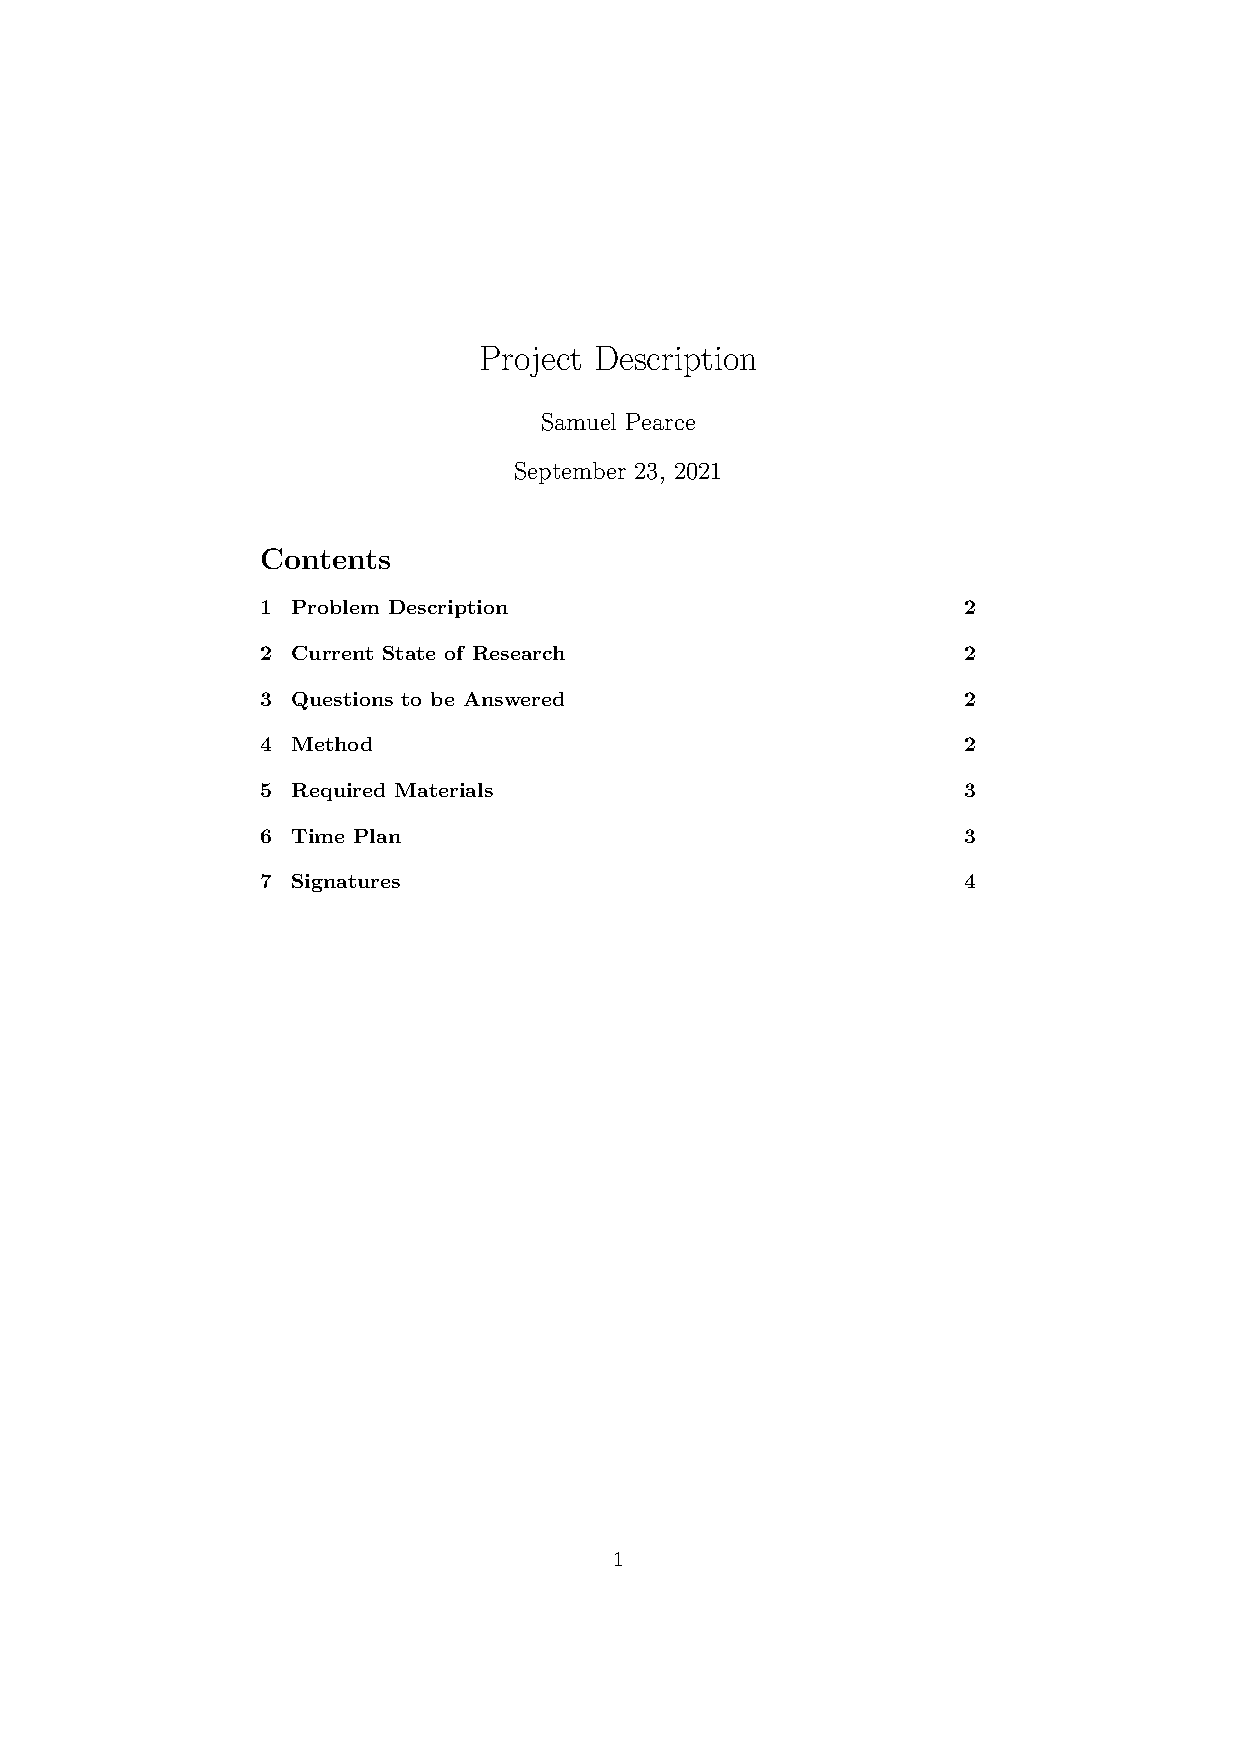
\includepdf[pages=-]{../Project_Description/Project_Description.pdf}

\section{Anhang B: Sutlun Grammatik und Lexikon}
\addcontentsline{toc}{section}{Anhang B: Sutlun Grammatikund Lexikon}
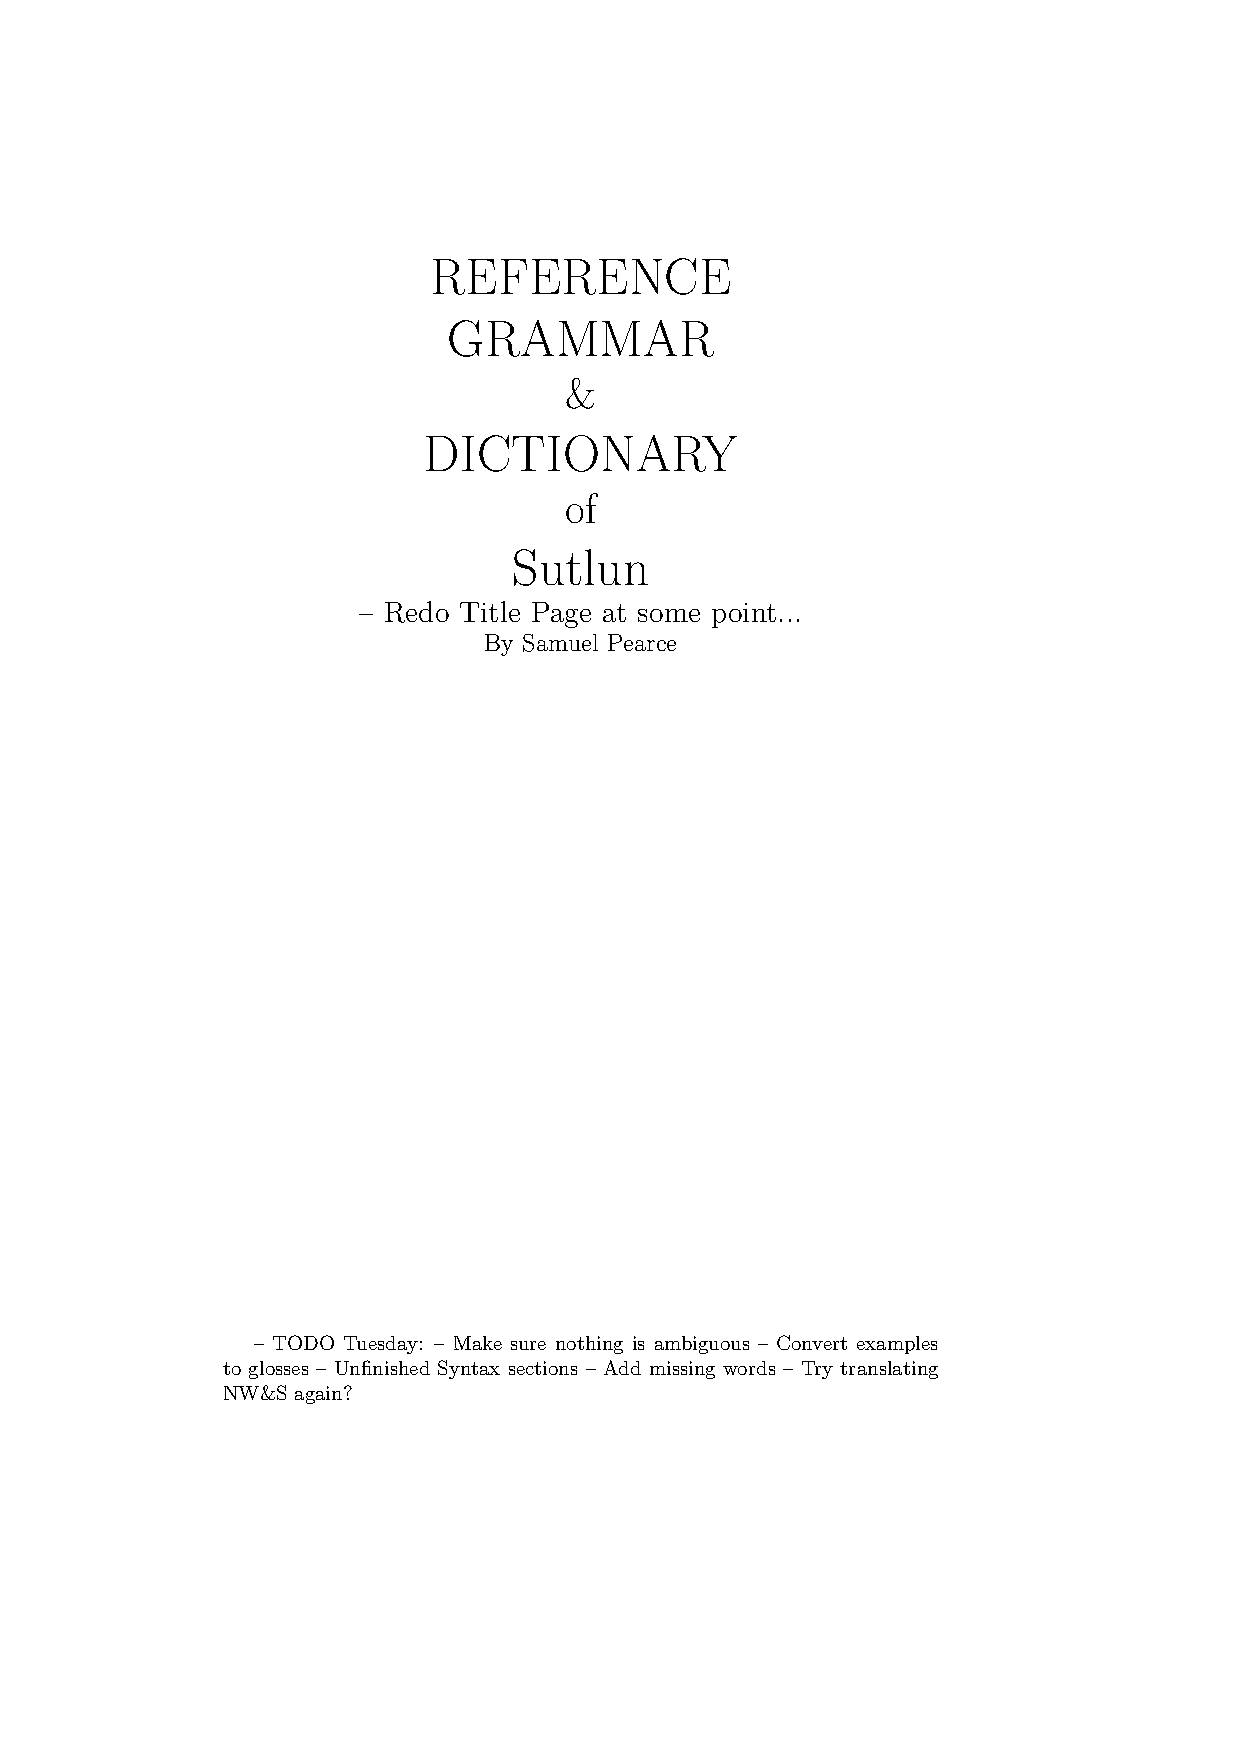
\includepdf[pages=-]{../Sutlun_Grammar/Sutlun_Grammar.pdf}

\section{Anhang C: Übersetzte Texte}
\addcontentsline{toc}{section}{Anhang C: Übersetzte Texte}
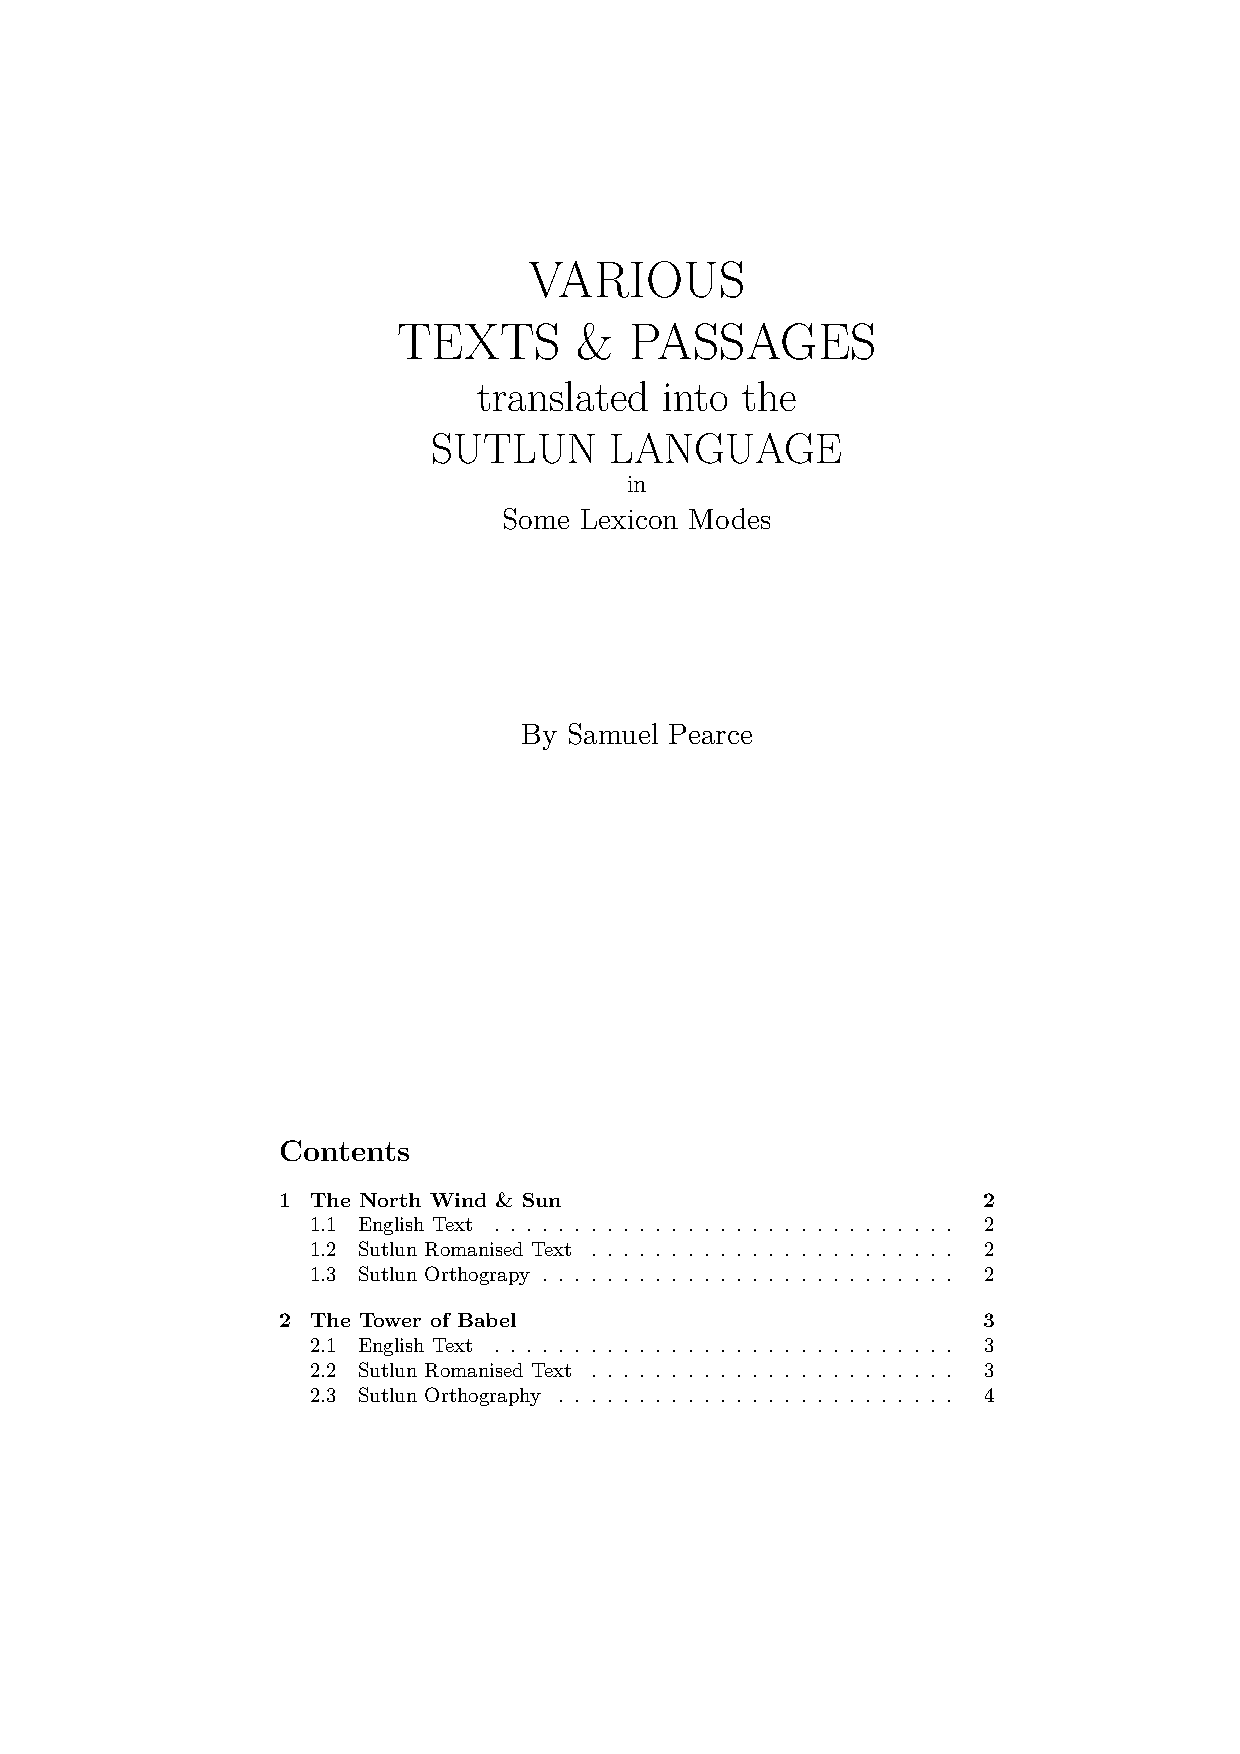
\includepdf[pages=-]{../Text_Translations/Text_Translations.pdf}

\section{Anhang D: Arbeitsprotokoll}
\addcontentsline{toc}{section}{Anhang D: Arbeitsprotokoll}
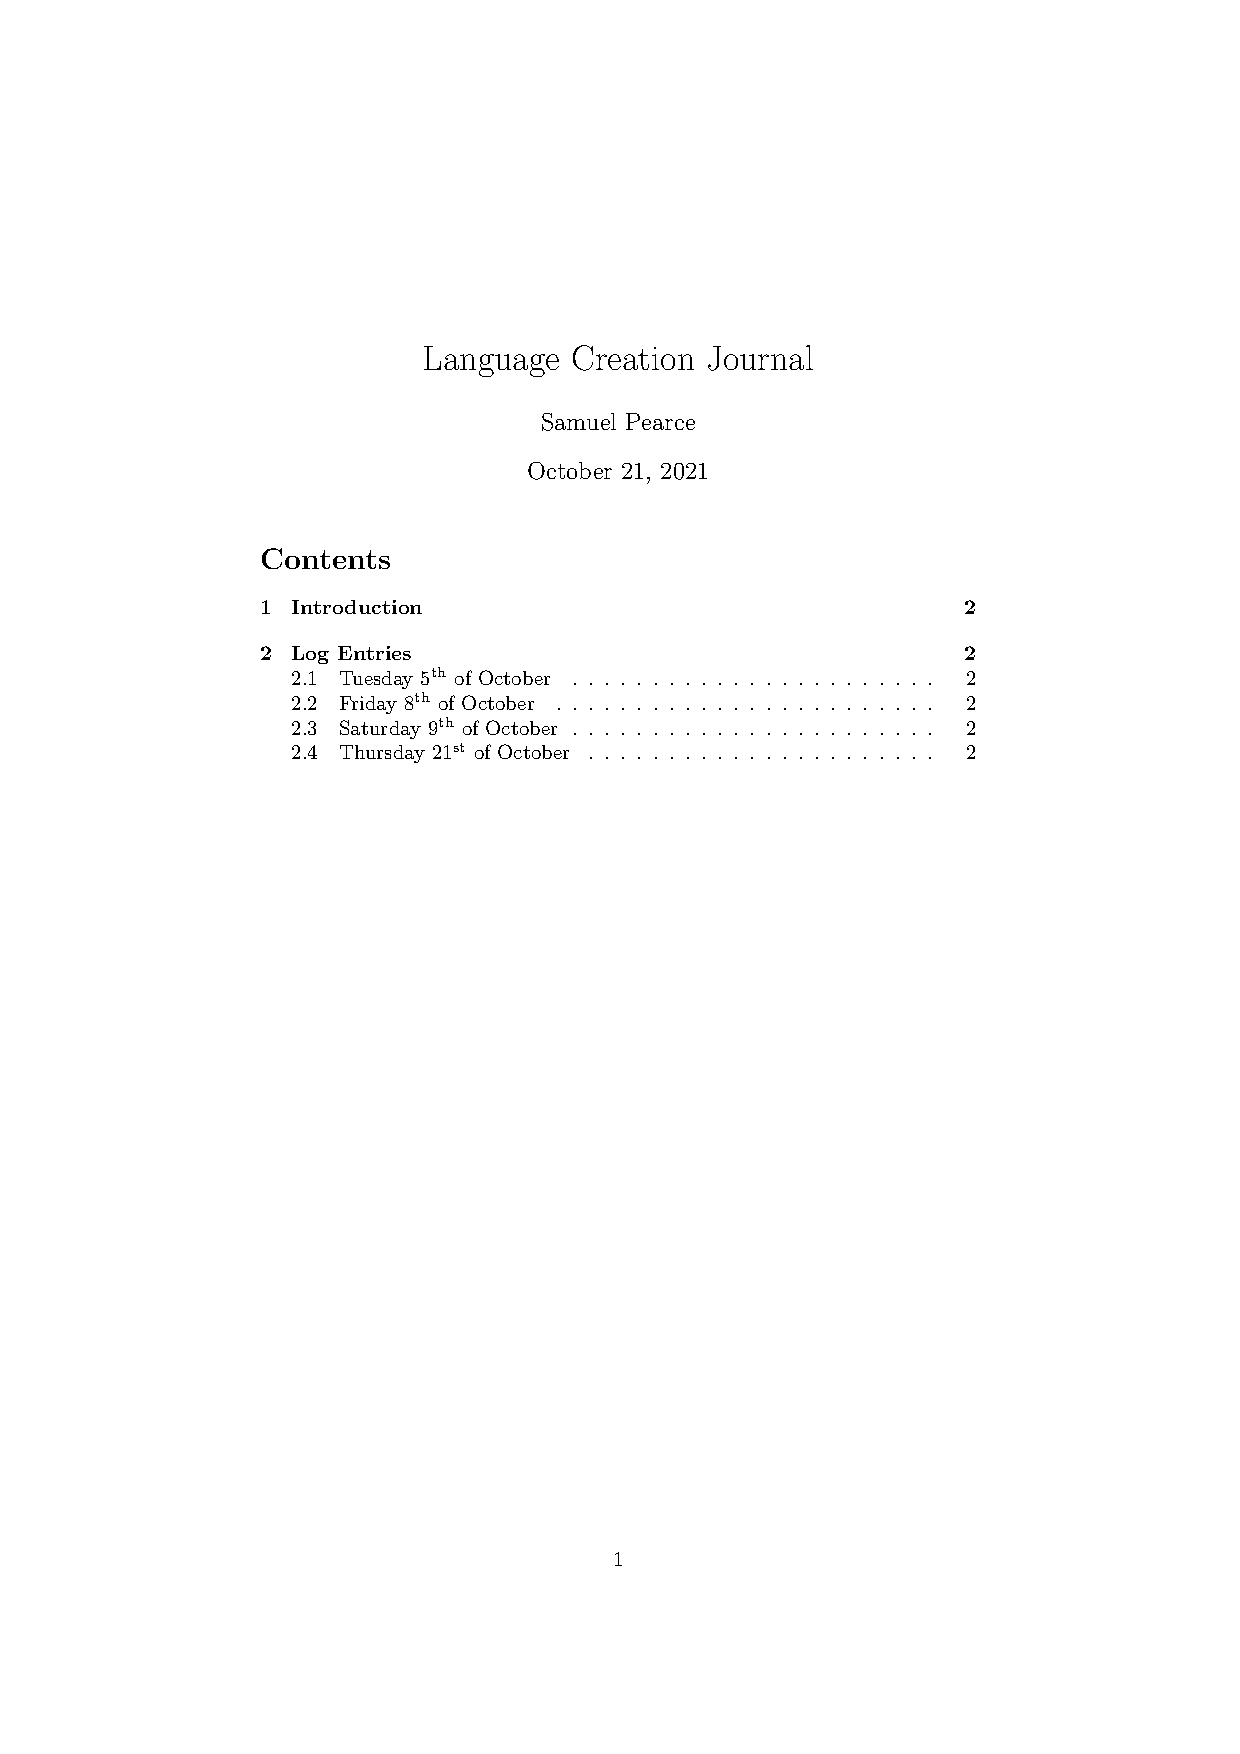
\includepdf[pages=-]{../Language_Log/langlog.pdf}

\section{Anhang E: Selbständigkeitserklärung}
\addcontentsline{toc}{section}{Anhang E: Selbständigkeitserklärung}
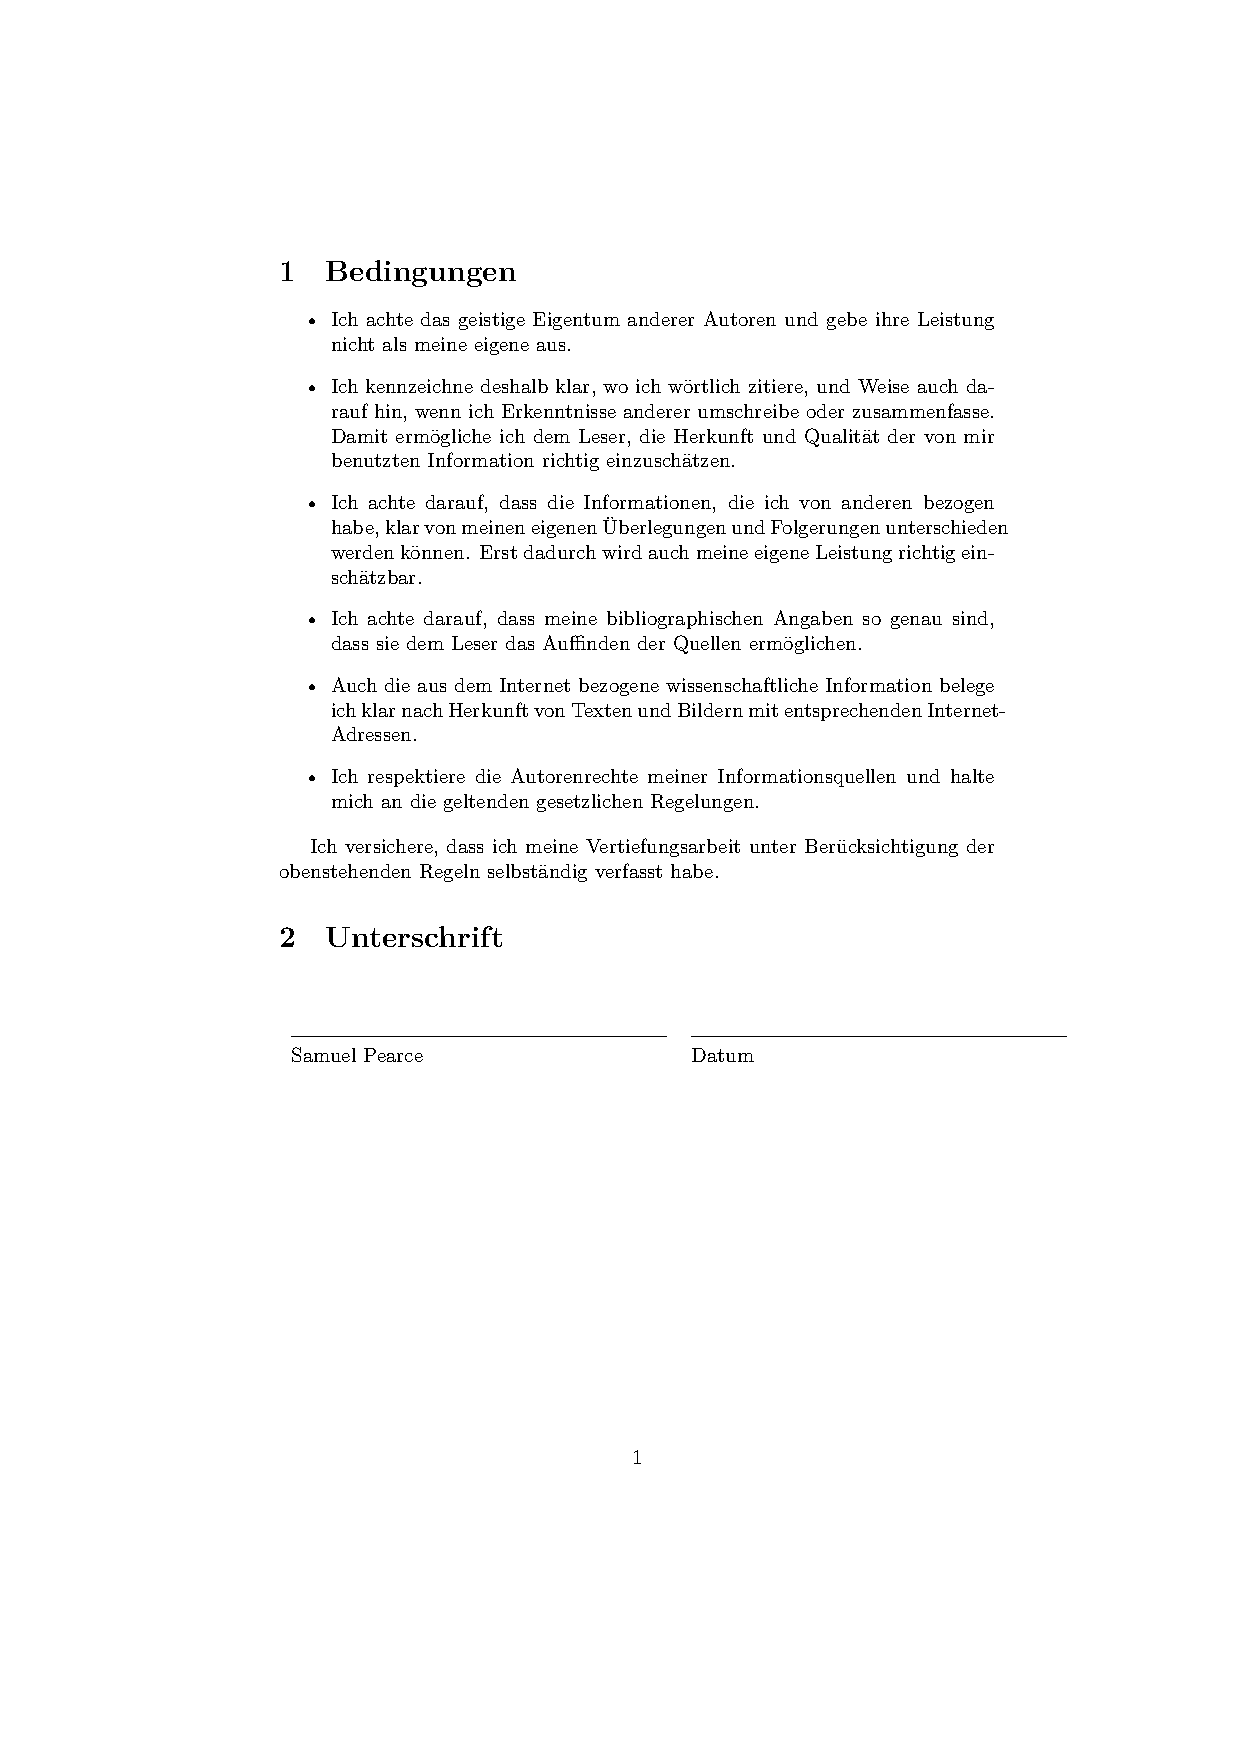
\includepdf[pages=-]{../Copyright_Declaration/Copyright_Declaration.pdf}

\end{document}